
% Due Date: 7/18/14

\chapter{Garbage Collection}
\label{chapter:garbage}
Many of the resources associated with a Legion application
are explicitly managed by the user.  For example, logical 
regions must be explicitly allocated and deallocated
by an application. However, while logical regions are 
explicitly managed by the application, the Legion runtime
is responsible for managing the allocation and freeing of
physical instances of logical regions. The reason for 
placing this responsibility on the runtime is a matter of
safety. If an application (or a mapper) had the ability
to explicitly allocate and deallocate physical instances
it could unsafely delete instances that are in use
or will be used by future tasks. Therefore, neither 
application code nor mapper objects are given permissions
to explicitly allocate or deallocate physical instances.
It is the responsibility of the runtime to explicitly 
manage physical instances and know when it is safe to 
reclaim them.

To support a safe reclamation scheme of physical instances,
the Legion runtime employs a garbage collection algorithm.
While there are many well known garbage collection 
routines for languages and runtimes, the one used
in the Legion runtime is unique. The novelty of our
approach stems from having to deal with two difficult
aspects of the Legion programming model.  First, garbage
collection in Legion must be capable of operating in 
a distributed environment because tasks may be mapping
to the same physical instance on different nodes.
Second, garbage collection in Legion must be capable
of operating within a deferred execution environment.
As we will show, our proposed garbage collection scheme
allows physical instances to be reclaimed and the
memory recycled even before the tasks using the
physical instances have started execution. Dealing with
these two different constraints has led us to a
garbage collection algorithm that differs in many
ways from traditional approaches.

The rest of this chapter is organized as follows:
in Section~\ref{sec:counting}, we give an overview
of the garbage collection algorithm and how it 
operates both within nodes as well as across nodes.
Sections~\ref{sec:distcollect} and \ref{sec:hiercollect}
describe the two different collection patterns that
comprise the basis for our garbage collection 
algorithm. Finally, in Section~\ref{sec:recycling},
we show how our garbage collection allows physical
instances to be safely recycled even before all the 
tasks using them have started running.

\section{Reference Counting Physical Instances}
\label{sec:counting}
To garbage collect physical instances, we rely
on existing data structures used for tracking
the usage of physical instances: instance managers
(described in Section~\ref{subsec:instmanagers})
and instance views (described in
Section~\ref{subsec:instviews}). Figure~\ref{fig:multigc}
provides an illustration for kinds of references kept
between the different components of the Legion runtime.
Both operations and physical states can maintain 
references to instance view objects. Instance view 
objects in turn maintain references to instance
manager objects. By using these existing data 
structures, we set up a two-level
reference counting scheme described in detail in
Section~\ref{subsec:twolevel}.
To further improve the efficiency
of our garbage collection algorithm, we also
track different kinds of references between
these data structures, allowing us to know
when a physical instance will eventually be
garbage collected, even though it may still be
some time before the instance is actually 
collected.  Different kinds of references permit
us to construct a two-tiered approach to reference 
counting for detecting these conditions in 
Section~\ref{subsec:twotier}.

\begin{figure}
\centering
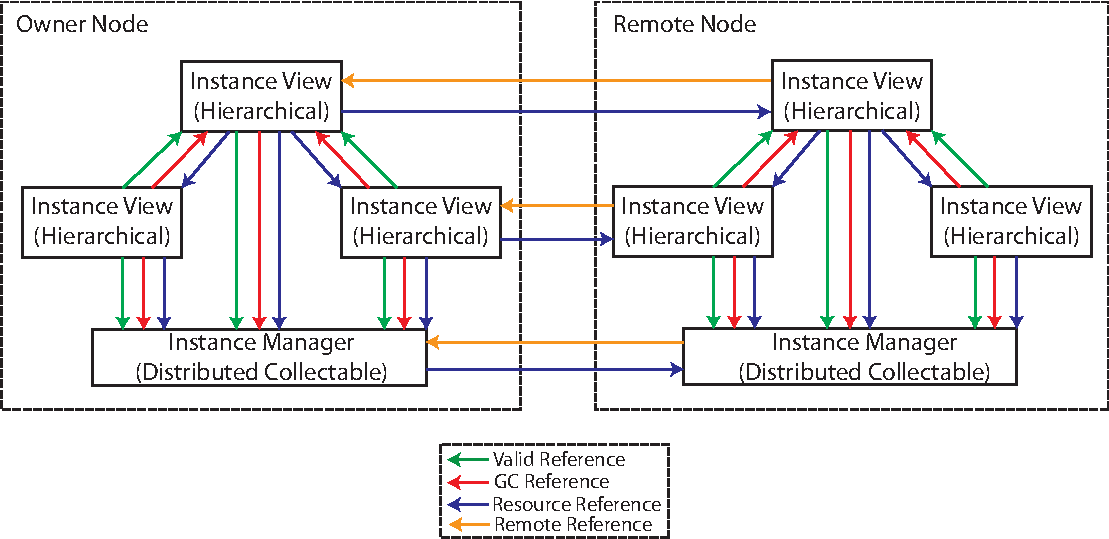
\includegraphics[scale=0.7]{figs/MultiNodeReference.pdf}
\caption{Legion Reference Counting Scheme\label{fig:multigc}}
\end{figure}

\subsection{Two-Level Reference Counting}
\label{subsec:twolevel}
In order to know that it is safe to garbage
collect a physical instance, the runtime must be
able to prove two conditions.  First, it must
be the case that there are no existing users of
a physical instance (either tasks or copies).
Second, the runtime must be able to show that 
there will not be any future users of the physical
instance. In both cases, the information for 
determining these conditions is available through
the instance view objects.  Instance view objects
record both the current users of a physical instance
from the perspective a given logical region in 
a context, as well as whether the instance view
contains valid data for any of the fields in the 
physical instance. Whenever an instance view either
has users of a physical instance or is a valid 
view, it adds a reference to the physical manager
with which it is associated to prevent the physical
instance owned by the manager from being collected.

Physical manager objects track all of the references
that they see from instance view objects on the node
in which they reside.  Recall from 
Section~\ref{subsec:instmanagers} that there is at
most one instance manager on a node for each
physical instance. This is a useful property to maintain
as it allows a single instance manager to be used
for tracking references from all instance views in
any physical context within a node. 

While a single instance manager on a node can track
references within the node, it cannot track references
to a physical instance between nodes. Only when all of
the nodes no longer have references is it safe to 
actually garbage collect the physical instance. To track
when it is safe to actually perform garbage collection
for a physical instance we use the {\em distributed
collectible} algorithm described in 
Section~\ref{sec:distcollect}. The distributed collectible
algorithm both tracks references between nodes and 
also aids in knowing when meta-data structures are safe
to free.

\subsection{Two-Tiered Reference Counting}
\label{subsec:twotier}
While maintaining references for purposes of garbage
collection is useful, it often represents a sub-optimal
approach to freeing memory in Legion's deferred execution
model. Garbage collection frees physical instances only
after they are no longer needed.  However, the Legion
programming model is based on the premise that mapping
will be occurring in advance of actual execution. When
mapping ahead of actual execution, it is possible in 
Legion to know that a physical instance will eventually
be collected well in advance of when the actual 
collection will occur. To detect these cases, we employ
two different {\em tiers} of reference counting: 
{\em valid references} for detecting when it is safe to 
{\em recycle} a physical instance, and {\em garbage 
collection} references for detecting when the instance can
actually be deleted. Based on the information provided
by this two-tiered reference counting approach, we can
free up the memory being consumed by the physical
instance in advance of the actual garbage collection,
thereby allowing additional tasks to map and further
hiding the latency of the mapping process.

We know that a physical instance will eventually be 
garbage collected once none of its instance views represent
valid versions of the data for any of the fields in the
physical instance. At this point, it is impossible for 
any new users to be registered with any of the instance 
view objects and the instance will ultimately be collected 
once all of the current users are done using it. To
detect this scenario, we differentiate the kinds of 
references that are kept between instance views and
instance managers. If an instance view contains valid
data, then it adds a valid reference to both its 
parent instance view (because that view is also valid)
and to the instance manager.  If an instance view has a user of
the physical instance then it adds a garbage collection 
reference to both its parent view and the instance manager. 
In order to recycle a physical instance before it has been 
collected, an instance manager only needs to prove that
there are no longer any valid references to the 
instance.  In order to perform garbage collection, a 
physical manager must be able to show that there are 
both no valid references and no garbage collection 
references. We discuss how the distributed collectible 
algorithm supports detecting these cases in a distributed
memory setting in Section~\ref{sec:distcollect}.

The two other kinds of references are {\em remote
references} and {\em resource references}. Remote references
represent aggregations of garbage collection references
for the distributed collectable and hierarchical collectable
objects discussed in Sections~\ref{sec:distcollect} and
\ref{sec:hiercollect}. Tracking only garbage collection
references and not valid references between nodes is an
important trade-off. Tracking valid references between nodes
would allow us to recycle instances that were known in 
distributed contexts. In practice, we have found that the cost
of performing tracking outweighs the performance benefits
and therefore we only track garbage collection references
between nodes with remote references for correctness.

Resource references allow us to track when the actual
meta-data objects themselves can be deleted. Resource 
references that are held by an object are only removed 
when an object itself is deleted. Resource references
are used to track when objects in higher tiers of the
collection scheme no longer require access to an object.
Similarly, resource references will also be used as 
part of the distributed and hierarchical collectable
algorithms to determine when objects on remote nodes
are safe to delete. 

\section{The Distributed Collectable Algorithm}
\label{sec:distcollect}
Performing reference counting garbage collection
in a distributed environment is a difficult 
proposition that requires a disciplined approach
to managing references between nodes in order to 
avoid incurring large inter-node communication 
overheads. Our approach to solving this problem 
is based a pattern that we call a {\em distributed 
collectable}. All nodes
that share access to a common resource maintain
a distributed collectable object for tracking
the usage of the resource.  By using a series
of different kinds of references, distributed
collectable objects can significantly reduce
the amount of reference counting communication
between nodes and discern when it is safe to
garbage collect a resource. The distributed
collectable pattern serves as the basis for
garbage collection of both physical instances
and distributed futures in the Legion runtime.

In this section we discuss the details of the 
distributed collectable algorithm. 
Section~\ref{subsec:distobjs} 
describes how distributed collectable objects
are created and organized on different nodes.
In Section~\ref{subsec:distmachine},
we cover the details of the distributed 
collectable state machine and how it allows
objects that inherit from it to make decisions
regarding the resource being managed.

\subsection{Distributed Collectable Objects}
\label{subsec:distobjs}
Distributed collectable objects are aggregators
of references within a node. Each node maintains
a unique distributed collectable object for 
a common resource (e.g. a physical instance).
Clients of the distributed collectable algorithm
can add two different kinds of references to
a distributed collectable object: {\em valid}
and {\em garbage collection}. These two kinds
of resources are described in detail in 
Section~\ref{subsec:twotier}. Importantly, by
grouping together these references within a
node, a distributed collectable object can 
summarize many references with a just a few
inter-node references and thereby significantly
reduce the amount of communication required
for performing inter-node reference counting.

While there may be multiple instances of a 
distributed collectable object throughout many
nodes on the system, one of these objects is
appointed the {\em owner}. When a resource is
allocated on a node, a distributed collectable
object is made to manage the resource and 
immediately becomes the owner. All other instances 
of the distributed collectable object on other 
nodes are considered {\em remote}. In order to
support communication between distributed
collectable objects managing the same resource,
each group of distributed collectable objects
are assigned a {\em distributed ID} that is
unique throughout the entire system. When a
distributed collectable object is created on 
a node, it registers itself with the runtime
using its assigned distributed ID. The 
distributed ID allows messages between 
distributed collectables on different nodes
to be properly routed by the runtime.

Figure~\ref{fig:distgc} illustrates an example
set of distributed collectable objects on 
different nodes for representing a common resource.
There are two kinds of references maintained
between distributed collectable objects on 
different nodes. First, all remote distributed
collectable objects add {\em remote} references
to the owner distributed collectable object
when they have at least one valid reference
or they have at least one garbage collection reference.
Note that this is an existence property: only
one remote valid reference is necessary to 
represent an arbitrarily larger number of 
valid references within a node. Adding a remote 
references requires sending a message from the 
remote distributed collectable object to the 
owner distributed collectable object. 
Ultimately, it is the owner 
object that makes the decision about when a resource 
can be recycled or garbage collected based on a 
combination of its local references as well
as remote reference. We discuss this process in
Section~\ref{subsec:distmachine}.

\begin{figure}
\centering
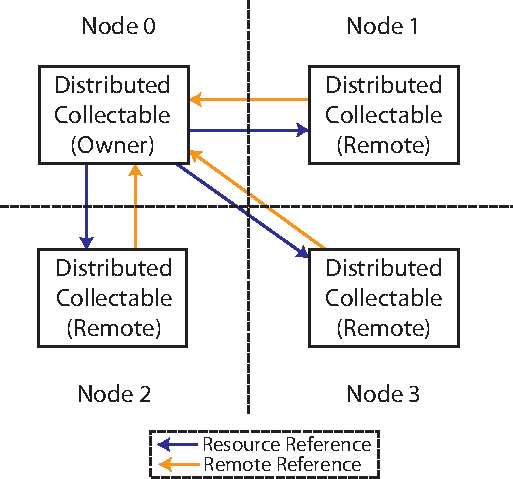
\includegraphics[scale=0.9]{figs/DistributedCollectable.pdf}
\caption{Distributed Collectable Example\label{fig:distgc}}
\end{figure}

The other kind of remote reference maintained
by the distributed collectable objects is
a {\em resource} reference.  A resource
reference is not used for direct garbage
collection, but instead is used for determining
when it is safe to actually delete the 
distributed collectable objects themselves.
Distributed collectable objects persist as
long as the resource they are managing
is still live. Once it has been reclaimed
then it is safe to free the distributed
collectable objects. The owner distributed
collectable maintains resource references
on all of the remote distributed collectable
objects. This is done implicitly without any
messages as the owner node can track which
remote instances it has heard from as part
of tracking references. Once a resource is
garbage collected, the owner distributed
collectable will first remove all its
resource references on the remote distributed
collectable objects and then free itself.
When the remote distributed collectable 
objects have their resource references 
removed, they know that it is safe to 
also free themselves.

One challenging part of the distributed 
collectable algorithm is the creation of a
new distributed collectable object on a remote
node. Each distributed collectable object
maintains a set describing which nodes it
already knows have instances of a distributed
collectable objects with the same distributed ID.
However, the algorithm permits these sets to 
be incomplete which may result in duplicate
sends of a creation request to the same node.
Since the runtime registers all distributed
collectable objects, it can detect when 
duplicate creation requests have been received
and ignore the additional requests.

The most difficult part of distributed
collectable creation is preventing premature
collections from happening while a creation
request is in flight. There 
are two possible scenarios: the owner node receives 
a request for remote creation and a remote node 
receives a request for remote creation. We handle 
each of these two cases in turn.

First, in the case where the owner nodes receives
the request to create a new remote distributed
collectable, it immediately adds a remote reference
to itself before sending off the message to the
remote node to perform the creation.
This additional reference guarantees that the 
owner node can not perform a collections
while the request is in flight. When the remote
distributed collectable is created on the remote
node, it is initialized as already having a remote
reference to the owner node.

The second case is more difficult and is illustrated
in Figure~\ref{fig:distcreate}. If a remote
distributed collectable $D$ receives a request to 
create a new distributed collectable on another
remote node $R$ it must ensure that the resource cannot
be collected while the creation request is in flight.
To achieve this, $D$ first sends a message to the 
instance of the distributed collectable on the owner node 
adding a remote reference on behalf of the soon-to-be-created
distributed collectable on $R$. After sending this message,
$D$ then sends a message to $R$, requesting
the creation of a new distributed collectable with
the same distributed ID. The reason this is sound
is because communication
channels between nodes are ordered (see
Section~\ref{subsec:channels}). We know that $D$ has
at least one remote reference on the owner. Any
request to remove this remote reference from the
owner will be ordered after the message sent to the owner
node adding the new remote reference for the distributed 
collectable being created in $R$.  Therefore, the total 
remote reference count on the owner node will remain 
greater than zero, and the resource will not be collected 
while the creation message is in flight.

\begin{figure}
\centering
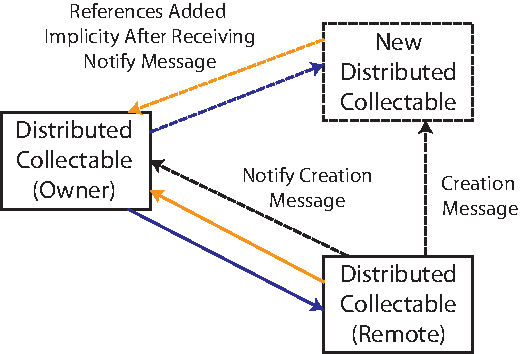
\includegraphics[scale=0.8]{figs/DistributedCollectableCreation.pdf}
\caption{Distributed Collectable Creation\label{fig:distcreate}}
\end{figure}

\subsection{Distributed Collectable State Machine}
\label{subsec:distmachine}
As part of its implementation, a distributed collectable
object keeps track of its state for the various kinds
of references that can be added and removed from it.
Figure~\ref{fig:diststate} shows an example of this
state machine. Distributed collectable objects traverse 
this state diagram monotonically dependent upon when valid
and garbage collection references are added or removed.
Distributed collectable objects start off in the initialized
stage and remain there until they receive their first 
valid or garbage collection reference. Once they receive
their first valid reference, they move into the valid and
referenced state. As soon as the number of valid references
returns to zero, then we know that the distributed
collectable object will eventually be collected. After
the number of garbage collection references, or remote references
representing garbage collection references, also drops
to zero, then we know that it is safe to actually 
collect the resource. It is the responsibility of the
client (in this case the rest of the Legion runtime)
to ensure that valid and garbage collection references
remain positive until the resource is no longer needed.
Failing to abide by this property can result
in double recycling or double frees of an application
resource.

\begin{figure}
\centering
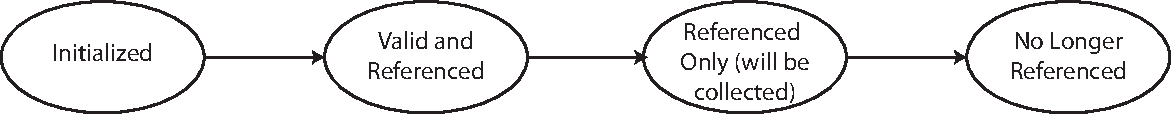
\includegraphics[scale=0.6]{figs/CollectableStateMachine.pdf}
\caption{Distributed Collectable State Machine\label{fig:diststate}}
\end{figure}

\section{The Hierarchical Collectable Algorithm}
\label{sec:hiercollect}
While the distributed collectable pattern is sufficient
for handling a flat distribution of objects across all
the nodes, it is insufficient for managing collections
of objects with a more complex sharing pattern. Consider
the case of instance view objects described in 
Section~\ref{subsec:instviews}. Instance view objects
are instantiated within a context and remote versions
of them whenever a context is sent remotely. Initially
this pattern of having an owner object and several
remote copies may seem similar to the distributed
collectable patter.  However, instance view management
is complicated by its interaction with virtual 
mappings (see Section~\ref{subsec:virtualmap}). With
virtual mappings it may be necessary for a remote
instance view itself to be sent remotely depending
on where tasks mapping within a virtual context are
sent. 

There are several different ways that we could handle
this case.  First, we could consider managing instance
views using the distributed collectable algorithm. 
This would be sufficient for knowing when it is safe
to add and remove valid and garbage collection references.
However, it would significantly complicate the update
pattern for adding users of instance views. Recall from
Section~\ref{subsec:invalidate} that the Legion runtime
uses an eager write-back, but lazy update model for
notifying instance views about new users. This means
that users must be eagerly sent back to an enclosing
physical context, but only lazily sent to other copies
of an instance view within the same context. If we
attempted to use the distributed collectable algorithm
here, the notion of the {\em owner} instance view 
would take on different values depending on the 
physical context. This would both complicate the 
garbage collection scheme as well as the bookkeeping
necessary to track which instance views needed to
be sent updates in different physical contexts.
Instead we chose to implement a different solution.

We call our alternative approach the hierarchical
collectable algorithm.  The general principle 
behind this garbage collection approach is that
each object in the scheme can act as both a remote
object as well as an owner object for its own
collection of remote objects. Unlike the distributed
collectable algorithm, the hierarchical collectable
algorithm makes no attempt to maintain uniqueness
of objects within a node.  In the hierarchical 
collectable algorithm there can be multiple copies
of the same object within a node.  While this may
seem redundant, the tree of hierarchical collectable
objects precisely captures the communication
network necessary for sending updates when virtual
mapped physical contexts are nested across several
remote nodes. Figure~\ref{fig:hiergc} shows an 
example of a hierarchical collectable object with
three different levels. Note that some instances
of the hierarchical collectable from different
levels are duplicated on the same node.

\begin{figure}
\centering
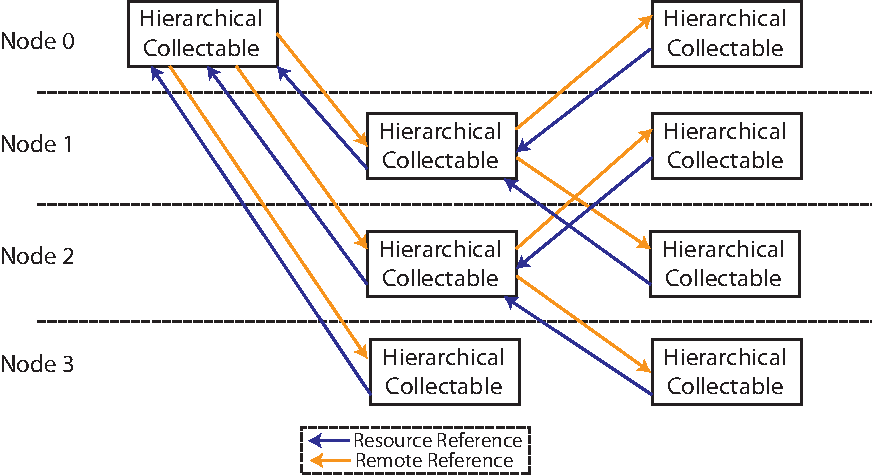
\includegraphics[scale=0.75]{figs/HierarchicalCollectable.pdf}
\caption{Hierarchical Collectable Example\label{fig:hiergc}}
\end{figure}

To implement the hierarchical collectable pattern,
each object is assigned a unique distributed ID.
(Note that this differs from the distributed collectable
pattern where all objects within a group are assigned
a common distributed ID.)  Copies of a hierarchical
collectable object can be requested on remote nodes.
Each hierarchical collectable object maintains a 
record of which nodes already have remote copies of
itself and the distributed IDs used to name those
copies on each remote node. When a new copy of a hierarchical
collectable is needed on a remote node, a message is sent
to the runtime on the target node requesting the
creation. The owner node allocates the distributed
ID and includes it in the creation message. The
creation of the remote version of the hierarchical
collectable object on the remote node then registers
itself with the runtime on that node, permitting the
same distributed ID based communication scheme used
by the distributed collectable objects.

In addition to sending the creation message to the
remote node, the owner also adds a remote reference 
to itself.  When the creation of the remote object
is complete, it already holds a remote reference to
the owner node ensuring that there is never any
premature garbage collection. This is 
simpler than the distributed collectable scenario
because only the owner node will ever create remote
copies of itself.

Any newly created hierarchical collectable object can 
then serve as an owner for its own set of remote copies. 
In the case of instance view objects, if the instance is 
in a physical context that is virtually
mapped, the runtime may create further remote
context copies that necessitate the creation of
additional hierarchical collectable objects on 
remote nodes. Since each hierarchical collectable
object keeps track of its own set of remote copies
there is no deduplication.

In order to perform garbage collection of the 
hierarchical collectable objects themselves, the
same resource reference approach is used as was
employed by the distributed collectable algorithm.
When the root of a hierarchical collectable tree
is garbage collected, it deletes itself and removes
all of its resource references on remote copies.
This process then results in the deletion of the
remote copies that recursively remove their 
resource references off of remote copies, ultimately
triggering the eventual reclamation of the entire
hierarchical collectable tree.


\section{Recycling Physical Instances in a Deferred Execution Model}
\label{sec:recycling}
The most novel aspect of the Legion garbage
collection scheme is that it permits safe recycling of 
physical instances before they are garbage collected.
Specifically, physical instances can be recycled as soon
as there are no longer any valid references to them.
As part of Legion's deferred execution model, it is 
possible that valid references to a physical instance
are all removed even before the instance is used by
an operation. By aggressively recycling physical instances, 
the Legion runtime can make more memory available
for operations to map, permitting greater run-ahead of
the deferred execution model and further hiding latency.

Recycling physical instances needs to be done in a 
disciplined way to avoid deadlock. When a physical instance
is recycled it is placed in a pool for physical instances
that are available for recycling. Each instance is also
marked indicating the depth in the task tree at which
the instance was allocated. To avoid deadlock, instances
are only able to be recycled for use with operations that
are at the same or a higher level of the task tree. 
This is an imprecise, but sufficient condition for guaranteeing
deadlock freedom. Consider the case where a parent task
$P$ maps a physical instance $I$.  As part of the execution
of $P$ it launches a child task $C$.  While $P$ was executing,
a sibling task of $P$ mapped causing the invalidation of all 
data in $I$, and thereby placing $I$ in the pool of instances to be recycled.
If $C$ then attempts to recycle the instance it is required
to wait on all previous users of $I$, including $P$.  When
$C$ must wait on $P$ we have a dependence cycle because
by definition $P$ must wait on $C$ to complete. By restricting
cycling to operations at the same or higher level of the
task tree we guarantee deadlock freedom. 

When a request to create a new physical instance is made as 
part of the physical dependence analysis 
(Chapter~\ref{chapter:physical}), the runtime
first checks to see if an instance is available in the
recycling pool that can be used. Currently, physical
instances are only allowed to be recycled if they exactly
match the memory usage of the requested physical instance.
This requires that the physical instance reside in the
requested target memory and the total memory usage be
identical. We require strict memory usage matching in 
order to avoid fragmentation that may result in memory
exhaustion and resource deadlock.

If an instance to recycle is found in the pool then it
is returned to satisfy the creation request. Before the 
physical instance is returned, it is assigned a 
{\em use event}, that is a merged event of all the 
termination events for all the current users of the physical 
instance in all of its instance views across all contexts. 
The use event becomes a precondition for any operation that 
uses the recycled physical instance to ensure that there are 
no data races for re-using the physical instance.

At some point the garbage collection for each physical
instance in the recycling pool will be triggered.  When this
occurs, the runtime checks to see if the physical instance
is still in the pool of physical instances eligible for
recycling. If it is, then the physical instance is removed
from the pool and then deleted, thereby returning the available
memory to the low-level runtime and preventing any future
recycling.  If the instance has already been recycled and
is in use by future operations then no action needs to occur.

Recycling of physical instances has some important implications
for the performance and memory usage of Legion programs. 
Recycling often permits the Legion runtime to map farther into 
the future as more memory resources appear to be available for 
mapping. Recycling of physical instances can also reduce the total 
memory usage of Legion applications as the same memory locations 
can be re-used for multiple tasks. While these effects of recycling
are often beneficial, they do come at the cost of sometimes
reducing the total amount of parallelism exploited by the
Legion runtime. Consider two non-interfering tasks $t_1$ 
and $t_2$.  If both tasks end up using the same physical 
instance with $t_2$ recycling an instance created by $t_1$,
then an event dependence is added between the two tasks
to prevent a race, reducing the total amount of parallelism
exploited. This trade-off between parallelism and memory
usage exists in many parallel programs and is primarily a
performance issue. As with all performance issues, we allow
applications to make decisions for themselves via the mapping
interface. By default recycling is enabled, but can be disabled
on a per region requirement granularity by setting a flag
on the region requirement as part of the {\tt map\_task}
mapper call. As part of future work we plan to investigate ways
of providing mappers a more global approach to mapping groups
of tasks so that they may better manage the trade-off between
memory usage and parallelism.

